\documentclass[a4paper]{report}

% \usepackage[utf8]{inputenc}
% \usepackage[T1]{fontenc}
% \usepackage{textcomp}
\usepackage[english]{babel}
\usepackage{amsmath, amssymb}
\usepackage[separate-uncertainty=true, multi-part-units=single]{siunitx}
\usepackage[]{subfig}
\usepackage[colorlinks=true, anchorcolor=blue, linkcolor=blue, citecolor=blue, bookmarks=false,hyperfootnotes=false]{hyperref}
\usepackage[margin=1in]{geometry}
\usepackage{color,soul}
\usepackage{tabularx}


% figure support
\usepackage{import}
\usepackage{xifthen}
\pdfminorversion=7
\usepackage{pdfpages}
\usepackage{transparent}
\usepackage{physics}
\graphicspath{ {./figures/} }
% \setlength{\parindent}{0pt}
\usepackage{chngcntr}
\usepackage{verbatim}
\usepackage{indentfirst}
\usepackage[most]{tcolorbox}
\usepackage{slashed}
\usepackage{listings}% http://ctan.org/pkg/listings
\lstset{
  basicstyle=\ttfamily,
  mathescape
}
\numberwithin{equation}{section}
\counterwithin{figure}{section}
\newcommand{\incfig}[1]{%
		\def\svgwidth{\columnwidth}
		\import{./figures/}{#1.pdf_tex}

}

\pdfsuppresswarningpagegroup=1

% for citations / references
\usepackage[style=ieee]{biblatex}
\addbibresource{atlas-report.bib}

\begin{document}

%----------------------------------------------------------------------------------------
%	TITLE PAGE
%----------------------------------------------------------------------------------------
\begin{titlepage} % Suppresses displaying the page number on the title page and the subsequent page counts as page 1
	\newcommand{\HRule}{\rule{\linewidth}{0.5mm}} % Defines a new command for horizontal lines, change thickness here
	
	\center % Centre everything on the page
	%------------------------------------------------
	%	Headings
	%------------------------------------------------
	
	\textsc{\LARGE Rheinische Friedrich-Wilhelms-Universit\"at Bonn }\\[4cm] % Main heading such as the name of your university/college
	
	\textsc{\Large Advanced Laboratory Course}\\[0.5cm] % Major heading such as course name
	
	\textsc{\large Performed on: May 23 - 24, 2022}\\[0.5cm] % Minor heading such as course title

	\textsc{\large Submitted on: June 2x, 2022}\\[0.5cm] % Minor heading such as course title
	
	%------------------------------------------------
	%	Title
	%------------------------------------------------
	
	\HRule\\[0.4cm]
	
	{\huge\bfseries E214: ATLAS}\\[0.4cm] % Title of your document
	
	\HRule\\[1.5cm]
	
	%------------------------------------------------
	%	Author(s)
	%------------------------------------------------
	
	\begin{minipage}{0.4\textwidth}
		\begin{flushleft}
			\large
			\textit{Authors}\\
			Keito Watanabe \\
			Paarth Thakkar
		\end{flushleft}
	\end{minipage}
	~
	\begin{minipage}{0.4\textwidth}
		\begin{flushright}
			\large
			\textit{Tutor(s)}\\
			Christina Dimitriadi
		\end{flushright}
	\end{minipage}

	\vspace*{5em}

	\begin{minipage}{0.8\textwidth}
		\begin{centering}
			% \large
			\textbf{Abstract}\\[0.2cm]
            
		\end{centering}
	\end{minipage}
	
	% If you don't want a supervisor, uncomment the two lines below and comment the code above
	%{\large\textit{Author}}\\
	%John \textsc{Smith} % Your name
	
	%------------------------------------------------
	%	Date
	%------------------------------------------------
	
	%\vfill\vfill\vfill % Position the date 3/4 down the remaining page
	% \vfill\vfill
	
	% {\large\today} % Date, change the \today to a set date if you want to be precise
	
	%------------------------------------------------
	%	Logo
	%------------------------------------------------
	
	%\vfill\vfill
	%\includegraphics[width=0.2\textwidth]{placeholder.jpg}\\[1cm] % Include a department/university logo - this will require the graphicx package
	 
	%----------------------------------------------------------------------------------------
	
	% \vfill % Push the date up 1/4 of the remaining page
	
\end{titlepage}

\tableofcontents

\chapter{Introduction} \label{chap:intro}

...
This report closely follows the student lab manual from \cite{labman}. All the constants for Standard Model (SM) particles were taken from \cite{ParticleDataGroup:2020ssz}. 

\chapter{Theory} \label{chap:theory}

\section{The Standard Model}
The Standard Model (SM) is one of the most tested theories in physics. It classifies all the known elementary particles into fermions and bosons and describes three of the four known fundamental forces of nature, strong, weak and electromagnetic force \cite{ParticleDataGroup:2020ssz}. The fermions are spin-1/2 particles and are further classified into quarks and leptons, each with three generations. The bosons are categorized by their spin with gluons, photons, $Z$ and $W^{\pm}$ boson having spin 1 and the higgs boson with spin 0. 

\chapter{LHC and the ATLAS Experiment} \label{chap:lhc_and_atlas}

\chapter{The Heavy Gauge Bosons} \label{chap:gauge_bosons}

\chapter{Pre-lab Questions} \label{chap:prelab}

\section{Part 2: Calibration of Electrons}

\noindent 1. Which value does the momentum of an electron have in the decay of a $Z^0$ boson $Z^0 \rightarrow e^+ + e^-$, if the $Z^0$ is at rest? 
\bigbreak
\noindent \underline{Solution}: \\
\noindent Given that the $Z^0$ boson is at rest, $\vec{p}_Z = 0 \implies E_Z^2 = \vec{p}_Z^2 + m_Z^2 = m_Z^2$ so that $E_Z = m_Z$. This implies that the 4-momentum of the $Z^0$-boson is $p_Z = (m_Z, \vec{0})$. 
\noindent Now by conservation of 4-momentum, we know that $p_Z = p_{e^+} + p_{e^-} \implies p_{e^+} = p_Z - p_{e^-}$. 

\noindent Now taking the dot product of $p_{e^+}$, we have that:
$$
p_{e^+} \cdot p_{e^+} = m_e^2 = (p_Z - p_{e^-}) \cdot (p_Z - p_{e^-}) = m_Z^2 + m_e^2 - 2 p_Z \cdot p_{e^-} = m_Z^2 + m_e^2 - 2m_Z E_e
$$
$$
\implies m_Z = 2E_e => E_e = \frac{m_Z}{2}
$$
\noindent where the property $(p \cdot p) = E^2 - \vec{p}^2 = m^2$ was used. 

\noindent To then determine the momentum of the electron, we use the energy-momentum relation again:
$$E_e^2 = \vec{p}_e^2 + m_e^2 \implies |\vec{p}_e| = \sqrt{E_e^2 - m_e^2} = \sqrt{\left(\frac{m_Z}{2}\right)^2- m_e^2}$$
$$\implies |\vec{p}_e| = \sqrt{\left(\frac{91.18 \text{GeV} }{2}\right)^2 - (5.11 \times 10^{-4} \text{GeV})^2} \approx 45.59 \text{GeV}$$

\noindent where the mass of the electron was neglected. 

\noindent Thus the momentum of the electron from a $Z^0$ boson decay at rest is $|\vec{p}_e| = 45.59 \text{GeV}$. 

\bigbreak

\noindent 2. How large is the momentum of tau leptons in the reaction $e^+ + e^- \rightarrow \tau^+ + \tau^-$, if the reaction takes place in the center-of-mass system (center-of-mass energy = 5 GeV)?
\bigbreak
\noindent \underline{Solution}: \\
\noindent We know that the mass of the tau lepton is $m_\tau = 1.776$ GeV. Given that the CoM energy is $\sqrt{s} = 5$ GeV, by conservation of energy we have that:
$$s = (2 E_e)^2 = (2 E_\tau)^2 = 4 (\vec{p}_\tau^2 + m_\tau^2) \implies |\vec{p}_\tau| = \sqrt{\frac{s}{4} - m_\tau^2}$$

$$
\implies |\vec{p}_\tau| = \sqrt{\frac{(5 \text{GeV})^2}{4} - (1.776 \text{GeV})^2} = 1.7595 \text{GeV}
$$

\section{Part 3.1: W-Boson Measurement}

\noindent 1. As before, the analysis is based on ROOT trees. One of the tree variables is $\texttt{ptw -}$  the estimated transverse momentum of the W boson candidate. This variable can be constructed from the other tree variables. Please think about how this could be done. The tree variables are listed in section B.
\bigbreak
\noindent \underline{Solution}: \\
\noindent Given that the weak interaction is described by $W \rightarrow l + \bar{\nu}_l$, we can calculate the transverse momentum of the W-boson from the transverse momentum of $l$ and $\bar{\nu}_l$.  The formula to evaluate this is:
$$p_{T_W} = \sqrt{p_{T_l}^2 + p_{T_\nu}^2}  $$
which is derived from the conservation of 3-momentum.

\noindent This is defined in ROOT as $\texttt{el\_pt} \ \text{and} \ \texttt{etmis}$, so that the transverse momentum of the W boson candidate can be calculated as such: $\sqrt{\texttt{el\_{pt}}^2 + \texttt{etmis}^2}$.

\bigbreak 

\noindent 2.  When fitting measurements to a linear function, the two parameters of a best fit straight line are y-intercept and slope. The errors on these parameters are typically correlated. Using these parameters for the error analysis will require a treatment that takes correlations into account. For example the simplest form of Gauss’ error propagation law requires that the errors are uncorrelated. Please look up the correct form of the Gauss error propagation law in the presence of correlations. You will need that for the final error on the W mass. On the other hand, is it possible to minimize correlations by choosing an appropriate coordinate system?
\bigbreak
\noindent \underline{Solution}: \\
\noindent The Gauss error propagation law in the presence of correlations is given as such:
$$
	\sigma_f ^2 = \left( \frac{df}{dx} \right)^2 \sigma_x^2 + \left( \frac{df}{dy} \right)^2 \sigma_y^2 + 2 \left( \frac{df}{dx} \right) \left( \frac{df}{dy} \right) \rho_{xy} \sigma_{x} \sigma_y $$
	
\noindent where $\rho_{xy}$ is the correlation coefficient which yields zero for uncorrelated errors. The correlation matrix is then defined with the variance $\sigma_x^2, \sigma_y^2$ in its diagonals with the correlations $\rho_{xy} \sigma_x \sigma_y$ in the off-diagonal components.

\noindent To minimize correlations, we can convert to an appropriate coordinate system in which the correlation matrix becomes diagonal. This will allow the cross terms to vanish.

\section{Part 3.2: New Physics}

\noindent 1. What is the minimum invariant 4-lepton-mass, when the four leptons originate from a $Z^0$ pair? Why do you find 4-lepton-events with invariant mass beneath this threshold?
\bigbreak
\noindent \underline{Solution}: \\
\noindent In theory, the minimum invariant mass of the each lepton should be $m_Z / 2$. In addition to the lowest order Feynman diagrams, there are two higher order diagrams where the photon is radiated by initial-state quarks, called Initial State Radiation (ISR), due to which there is a shift in the energy of the ingoing particles, leading to a distortion in the shape of the $Z$ resonance curve. Therefore, the effect of ISR is reduce the effective centre-of-mass energy of the ingoing particles, which leads to some fraction of $Z$ boson invariant mass to be beneath this threshold. 
Another possible reason can be that in the case of more than one Z boson, the other Z boson will not be on-shell due to kinematic reasons. Due to this, we get one Z boson and another virtual Z* boson. Hence, the mass of the 4 leptons, would be below the threshold. 

\bigbreak

\noindent 2. Consider a Higgs boson which decays into two $Z^0$ bosons. How does the distribution of the 4-lepton-invariant-mass look like?
\bigbreak
\noindent \underline{Solution}: \\
\noindent The distribution will follow a Voigt function peaked at ~125 GeV (Fig. \ref{fig:higgs-decay}).

\begin{figure}[htpb]
    \centering
    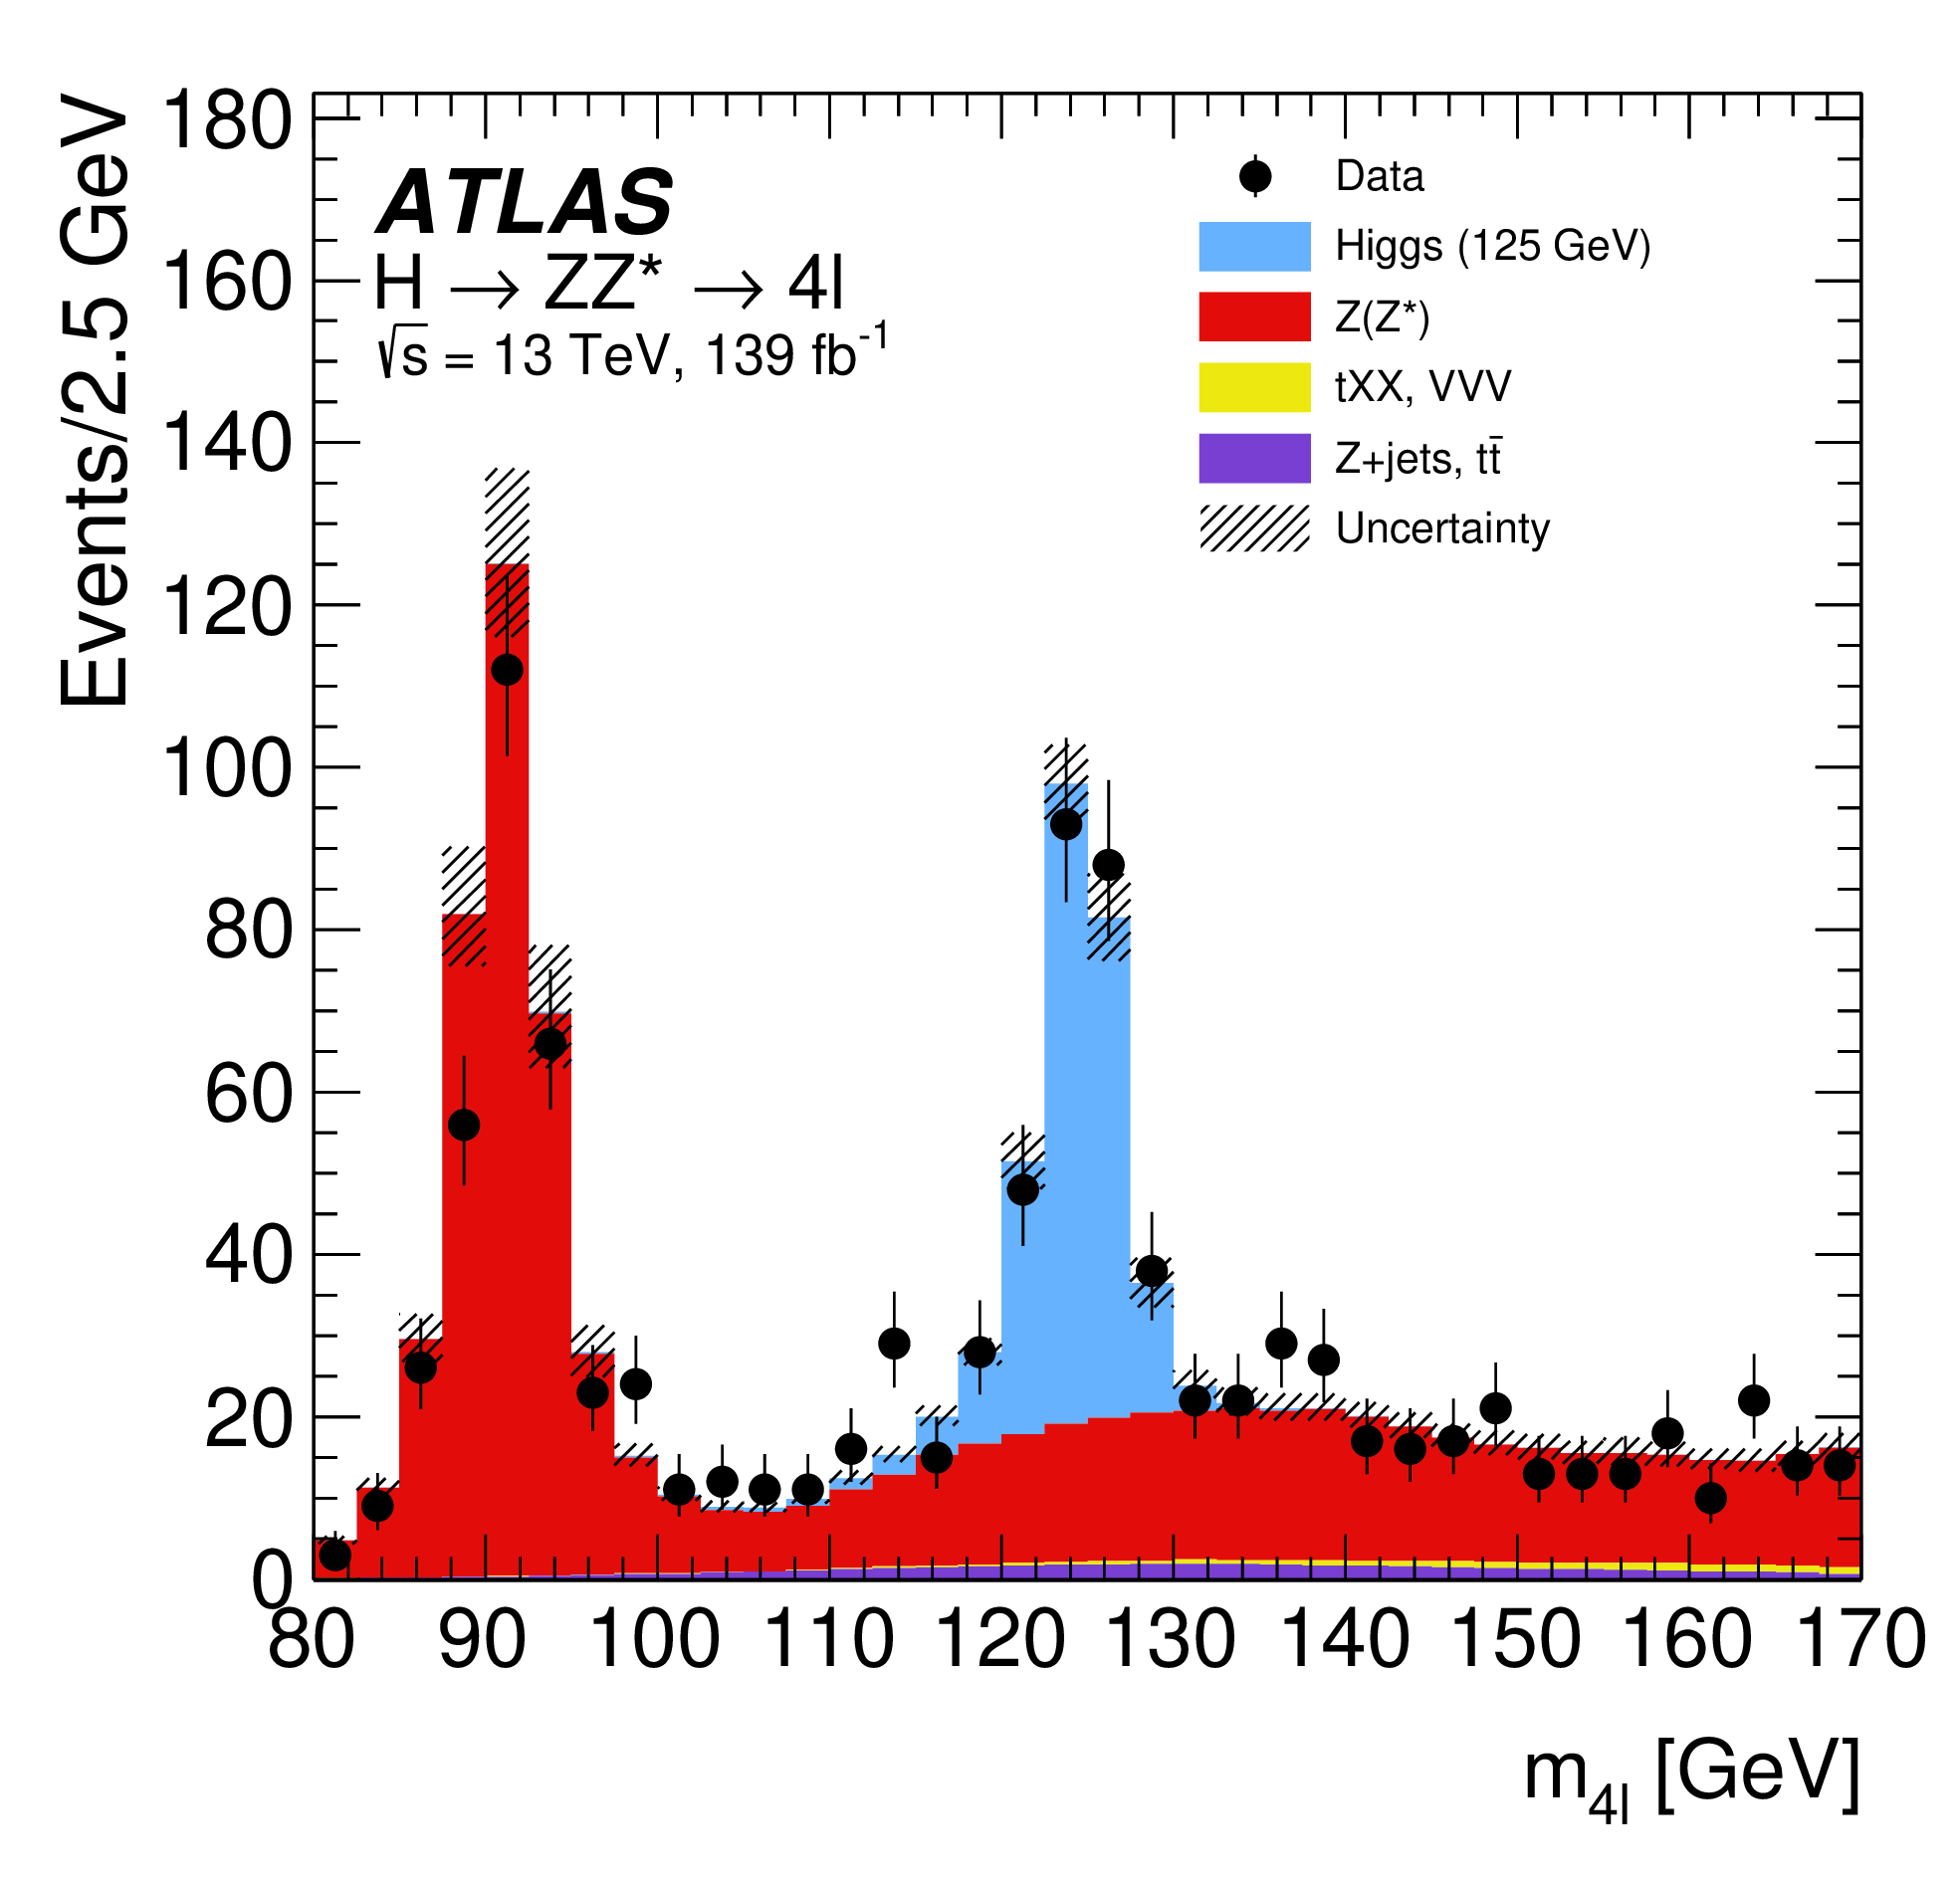
\includegraphics[width=0.6\textwidth]{higgs-decay}
    \caption{Higgs decay process \cite{ATLAS:2020wny}.}
    \label{fig:higgs-decay}
\end{figure}

\bigbreak

\noindent 3. Assume you have an ideal detector. What is the typical $\slashed{E_T}$ if a $Z^0$ pair has been produced and both $Z^0$ decay into electron or muon pairs? What $\slashed{E_T}$ will you expect when you have a real detector?
\bigbreak
\noindent \underline{Solution}: \\
\noindent In an ideal case, the expected $\slashed{E_T}$ is 0. In the case of real detector, $\slashed{E_T}$ will be non-zero due to inefficiencies in the detector and reconstruction algorithms. Further, not all muons and electrons will be detected. Or, one of the leptons could be extremely soft and not be detected at all. 

\bigbreak

\noindent 4. The Branching ratio of $t \rightarrow W b$ is almost 100\%. If you have a top anti-top pair in an event, both particles decay instantly via $t \rightarrow W b$. If both W bosons each decay leptonically ($W \rightarrow l \nu$), one finds two leptons in the event. What could explain the occurence of four leptons in a $t \bar{t}$ event?
\bigbreak
\noindent \underline{Solution}: \\
\begin{itemize}
	\item One of the leptons radiates a photon/Z* boson which gives lepton-antilepton pair, $l \rightarrow l + \gamma \rightarrow l + l^+ + l^-$.
	\item b-quark can decay semi-leptonically, giving us hadrons plus a lepton (Fig. \ref{fig:bdecay}).
\end{itemize}

\begin{figure}[htpb]
    \centering
    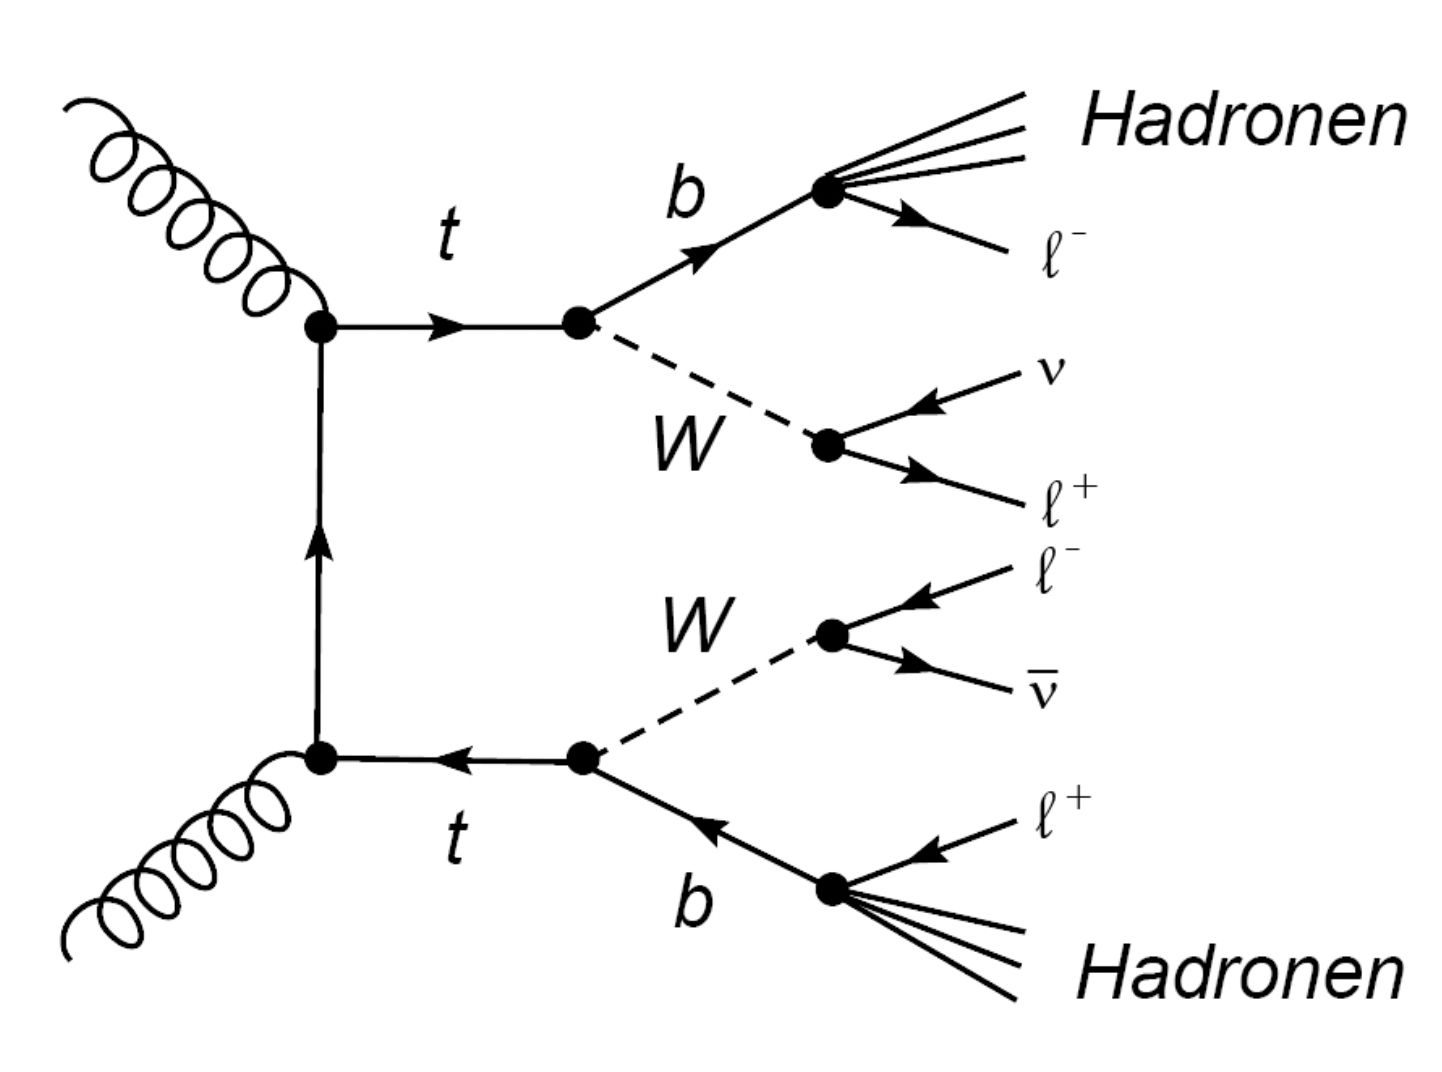
\includegraphics[width=0.6\textwidth]{bdecay}
    \caption{Top and b-quark decay process \cite{labman}.}
    \label{fig:bdecay}
\end{figure}

\chapter{Analysis} \label{chap:analysis}

\section{Part 1: ATLANTIS} \label{sec:atlantis}

In this part of the lab, we get familiar with the program \texttt{ATLANTIS}, which displays particle reactions in the ATLAS detector, graphically. 
...

Next, we work with two of the assignments listed in the lab manual. Since we were allowed to pick the assignments on our own, we choose to work with the \texttt{mystery-035-f.dat} data set and \texttt{xxx.dat} data set. 

\subsection{Mystery Data set}
In this data set, a pre-selection is applied, in which at least two leptons ($e$ or $\mu$) are required to be in each event. The goal of this exercise is to look at the graphics and identify various Standard-Model processes by studying them. Further, we must try to rule out certain processes, if any. In Fig. \ref{fig:mys1}, we see the graphical view of event 13. Fig. \ref{fig:mys1_2}, gives us the zoomed in view of the vertex for the same event. We start our discussion from the vertex. 

A zoomed in view of the vertex shows that most tracks originate from the vertex, but some a reasonably far away from the vertex. The tracks originating far away from the vertex must come from a particle which has decayed after a certain period of time. This gives us the following three possibilities for the original particle: $\tau^{\pm}$ lepton, top quark or b-quarks (b-jet). Since $W$ and $Z$ boson decay almost immediately, the track reconstruction resolution would not be able to pick on the slight differences in the vertex due to those decays. 

As these particles start heading towards the detector, we see that charged particles are bent based on their momentum and leave a ``hit'' in the inner detector. Some particles are too ``soft'' and hence their tracks disappear before reaching the ECAL. Looking at the deposition at the ECAL and HCAL, we see that most depositions between them align with each other. This indicates the presence of charged electrons and photons in jets. We know that b-jets contain leptons, as in 25\% of all B decays, a lepton is produced. We can get this b-quark from the top quarks via $t \rightarrow W^+ b$. The figure in the bottom half also shows the presence of isolated jets, without leptons. Since $\tau$ leptons can decay purely to hadrons and neutrinos, one of the ways to identify them is to look for collimated ``mini'' jets. 
 
Two other interesting tracks we see in the ECAL and HCAL are the isolated depositions in ECAL which do not have a corresponding deposition in the HCAL. This means that these charged electrons can come from the following sources: photons, $W$ bosons, $Z$ bosons and $\tau$ leptons. The presence of missing energy in the event confirms the existence of neutrinos and hence, confirms the possibility of $W$ boson decays. The other interesting track corresponds to the deposition in HCAL and then a track in the muon detector. This confirms the presence of muons in the event, which was probably surrounded by jets. Ths could be either due to top quarks or b-quarks. 

\begin{figure}[htpb]
    \centering
    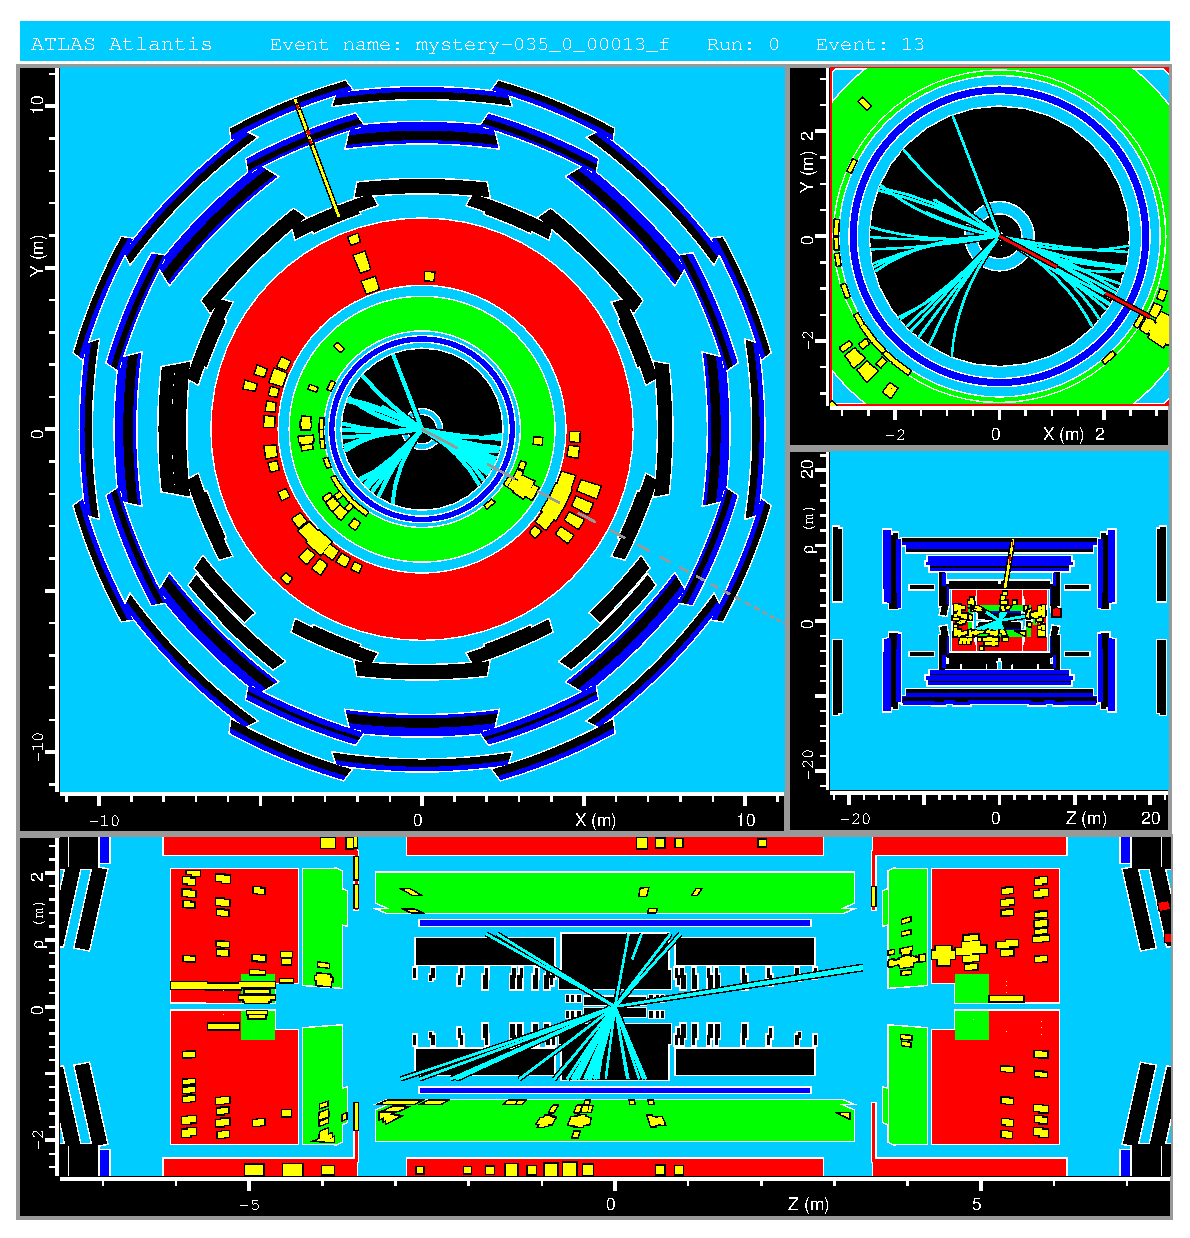
\includegraphics[width=0.6\textwidth]{mystery-035_0_00013_f-YX-RZ-RZ-YX-2022-05-23-13-28-39}
    \caption{Event name: \texttt{mystery-035-f}, Event: 13.}
    \label{fig:mys1}
\end{figure}

\begin{figure}[htpb]
    \centering
    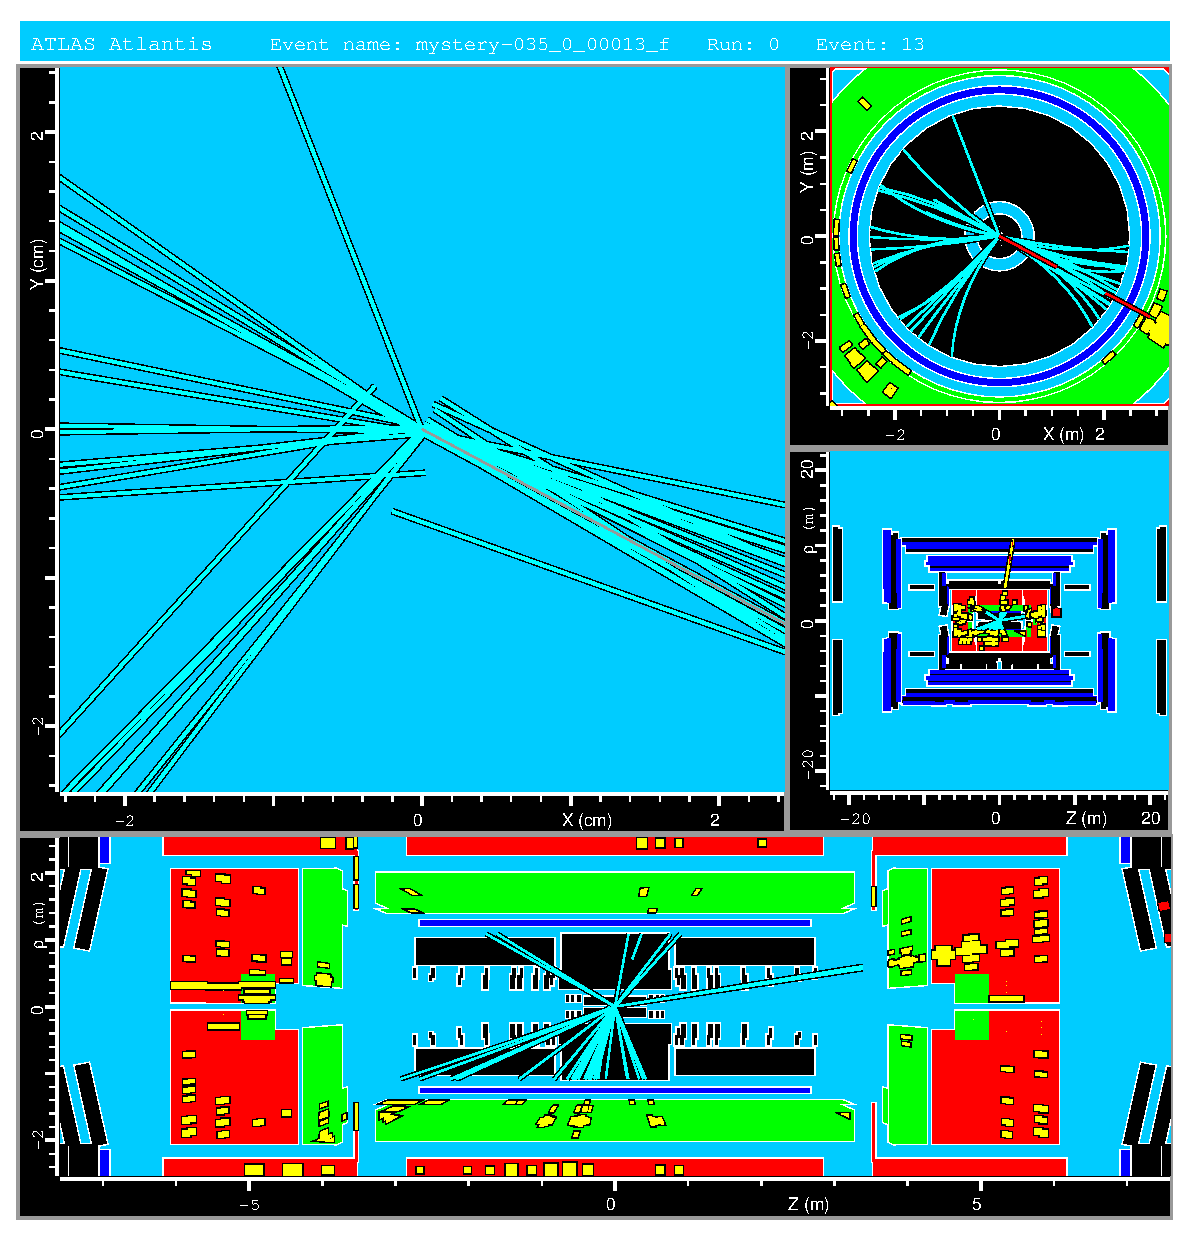
\includegraphics[width=0.6\textwidth]{mystery-035_0_00013_f-YX-RZ-RZ-YX-2022-05-23-13-34-34}
    \caption{Event name: \texttt{mystery-035-f}, Event: 13.}
    \label{fig:mys1_2}
\end{figure}


We look at one more event in Fig. \ref{fig:mys3}, event 12. In this event as well, we see all of the properties discussed above. Some thing which are slightly different is a higher number of isolated deposits in ECAL (without the corresponding deposit in HCAL) and the presence of two muons instead of a single one, both in the presence of jets. By selecting the missing energy track, we can look at the numbers. The following output was shown in the terminal: 

\begin{lstlisting}
ETMis:
 storegate key: MET_Final
 Sum-ET  = 1087.585 GeV
 ET-Mis  = 30.292 GeV
 ETx-Mis = -30.055 GeV
 ETy-Mis = 3.781 GeV
 $\phi$ = 172.829$^{\circ}$
 \end{lstlisting}

Since the $\slashed{E_T}$ is quite high, we can confirm the existence of one or more neutrinos in the event. Based on the discussion above, it is not possible to rule out any SM process for two lepton events. 


\begin{figure}[htpb]
    \centering
    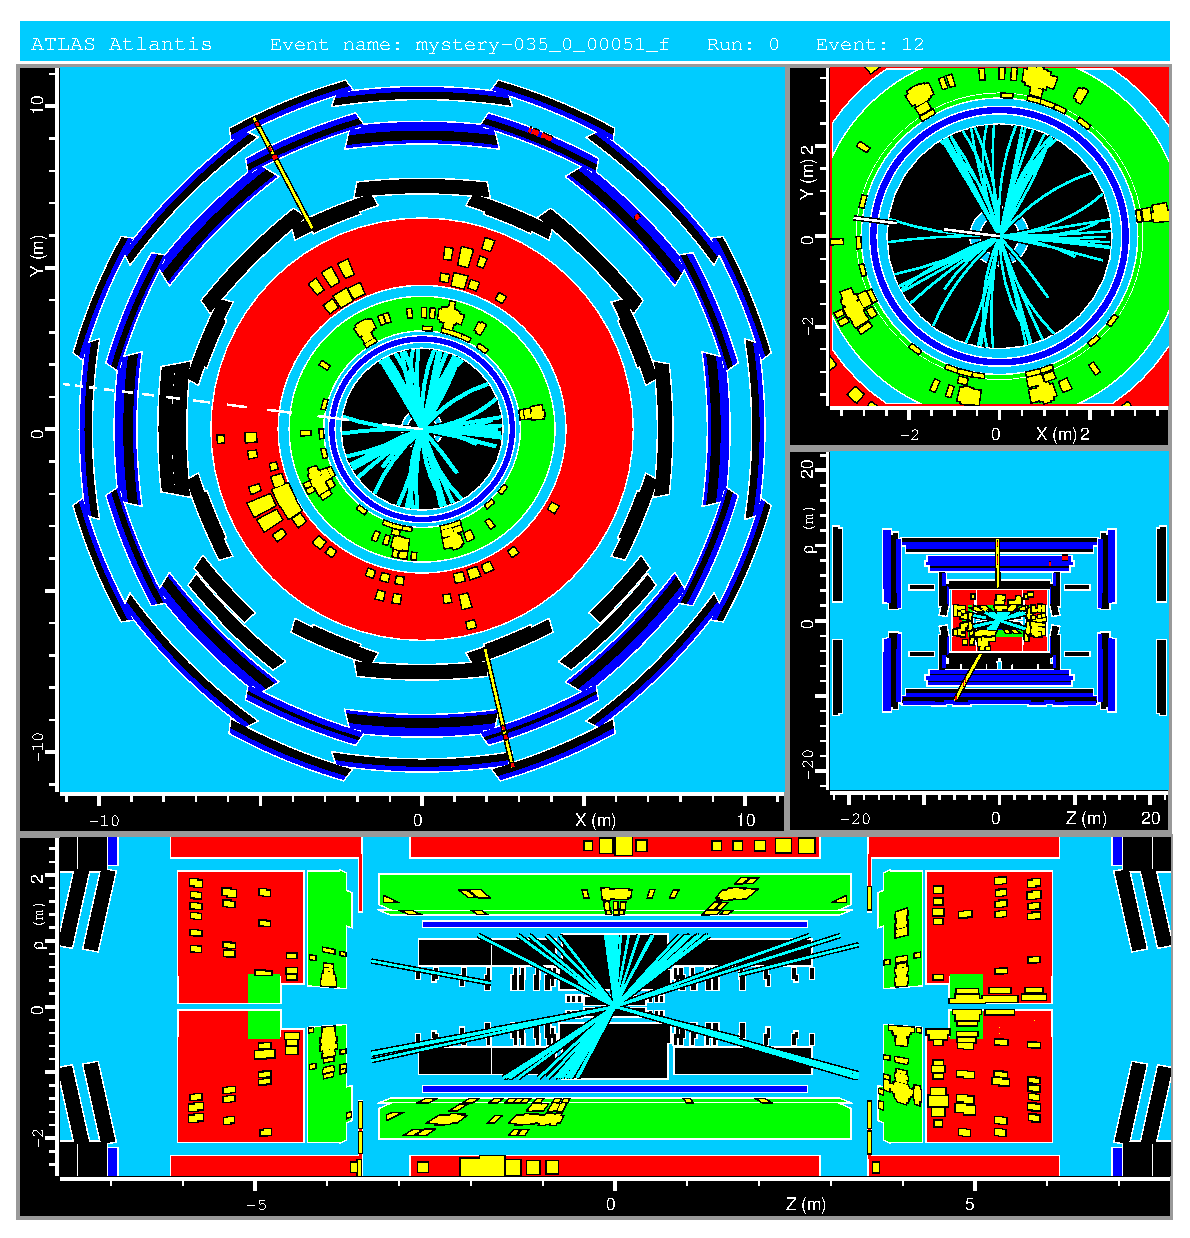
\includegraphics[width=0.6\textwidth]{mystery-035_0_00051_f-YX-RZ-RZ-YX-2022-06-18-17-20-41}
    \caption{Event name: \texttt{mystery-035-f}, Event: 12.}
    \label{fig:mys3}
\end{figure}

\printbibliography

\end{document}
